%
% Einfache LaTeX-Vorlage f�r Arbeiten am Lehrstuhl Kranzlm�ller / MNM-Team
% - optimiert f�r die Arbeit mit g�ngigen LaTeX-Editoren
% - funktioniert ohne Makefile und Anpassungen der LaTeX-Verzeichnisstruktur
% - verwendet Komaskript f�r ein (nach europ�ischen Gepflogenheiten) sch�neres Layout
% 
% v1, 2007 (Michael Brenner)
% Diese Version: v1.1, 2012 (Michael Brenner)
%


\documentclass[bibliography=totoc,listof=totoc,BCOR=5mm,DIV=12]{scrbook} % Rand f�r Bindung: 5mm / falls Index verwendet, erg�nze "index=totoc" zu den Optionen 
% \usepackage{bibgerm}       % deutsche Literaturverzeichnisse
\usepackage[latin1]{inputenc} % Umlaute im Text
\usepackage{graphicx} % Einf�gen von Grafiken  - f�r PDF-Latex: .pdf und .png (.jpg m�glich, sollte aber vermieden werden)
\usepackage{mathtools}		% sch�nere Summenzeichen usw
\usepackage{mathrsfs}		% kursive Buchstaben
\usepackage{url}           % URL's (z.B. in Literatur) sch�ner formatieren
\usepackage{hyperref} % sorgt f�r f�r Hyperlinks in PDF-Dokumenten
%\usepackage{cite}
\usepackage[noadjust]{cite}
\graphicspath{{./Bilder/}}

%
% der Befehl \hypenation versteht keine Sonderzeichen, also weder �
% noch "a noch \"a. W�rter die derartige Zeichen enthalten m�ssen
% direkt im Text getrennt werden, z.B. W�r\-ter
%
\hyphenation{Ma-nage-ment}
\hyphenation{Ma-nage-ment-agent}
\hyphenation{Ma-nage-ment-agent-en}
\hyphenation{Ma-nage-ment-ar-chi-tek-tur}
\hyphenation{Ma-nage-ment-ar-chi-tek-tu-ren}
\hyphenation{Ma-nage-ment-an-wen-dung}
\hyphenation{Ma-nage-ment-an-wen-dung-en}
\hyphenation{Ma-nage-ment-an-for-der-ung}
\hyphenation{Ma-nage-ment-funk-ti-on}
\hyphenation{Ma-nage-ment-funk-ti-onen}
\hyphenation{Ma-nage-ment-kon-zep-te}
\hyphenation{Ma-nage-ment-res-source}
\hyphenation{Ma-nage-ment-in-for-ma-ti-on}
\hyphenation{Ma-nage-ment-res-sour-cen}
\hyphenation{ma-nage-ment-re-le-vante}
\hyphenation{ma-nage-ment-sy-stem}
\hyphenation{ma-nage-ment-sy-steme}
\hyphenation{Ma-nage-ment-in-stru-men-tie-rung}
\hyphenation{Ma-nage-ment-platt-form}
\hyphenation{Sys-te-men}
\hyphenation{Sys-tem-um-ge-bun-gen}
\hyphenation{Sys-tem-ma-nage-ment}
\hyphenation{DHCP}
\hyphenation{Ma-nage-ment-diszi-plinen}
\hyphenation{System-management-architekturen}
\hyphenation{Verwendungs-nachweise}
\hyphenation{Video-einricht-ungen}
\hyphenation{Res-source}
\hyphenation{Res-sourcen}
\hyphenation{Grund-anwendung}
\hyphenation{Grund-anwendungen}
\hyphenation{Basis-anwendung}
\hyphenation{Core}
\hyphenation{Kom-mu-ni-ka-ti-on}
\hyphenation{De-sign-ent-schei-dung}
\hyphenation{Sprung-ad-res-sen}
\hyphenation{Klas-si-fi-ka-ti-on}
\hyphenation{Schreib-recht}
\hyphenation{Be-nut-zer-zer-ti-fi-kat}
\hyphenation{Bau-stein-ent-wi-ckler}
\hyphenation{ad-mi-ni-stra-ti-ve}

 % in dieses File kommen W�rter die Latex nicht richtig trennt

\begin{document}

% ---------------------------------------------------------------
\frontmatter % Titelbl�tter und Erkl�rung jeweils spezifisch f�r die jeweilige Uni einbinden
    %%%%%%%%%%%%%%%%%%%%%%%%%%%%%%%
% erste Seite

\thispagestyle{empty}

\begin{center}

\vspace*{-2cm}

{\Huge INSTITUT F�R INFORMATIK\\[1mm]}
DER LUDWIG--MAXIMILIANS--UNIVERSIT�T M�NCHEN\\

\vspace*{1cm}


\includegraphics[width=0.3\textwidth]{lmu_siegel}

\vspace*{2cm}

{\Large \textbf{Master's Thesis}}\\ % oder Fortgeschrittenenpraktikum, Master's Thesis, Bachelorarbeit etc.

\vspace{2.0cm}
{\Huge \textbf{Evaluation of Virtual Reality based Mesh Saliency Maps}}\\
% \vspace*{3mm}
% {\Huge \textbf{-- additional line}}\\
\vspace{1.5cm}

{\LARGE Richard Metzler} % Name des Autors

\vspace{3cm}
Draft vom \today % erleichtert den Betreuern die Zuordnung - f�r finale Version entfernen

\end{center}

\newpage

%%%%%%%%%%%%%%%%%%%%%%%%%%%%%%%
% zweite Seite

\thispagestyle{empty}
\cleardoublepage

%%%%%%%%%%%%%%%%%%%%%%%%%%%%%%%
% dritte Seite (Kopie der ersten)

\thispagestyle{empty}

\begin{center}

\vspace*{-2cm}

{\Huge INSTITUT F�R INFORMATIK\\[1mm]}
DER LUDWIG--MAXIMILIANS--UNIVERSIT�T M�NCHEN\\

\vspace*{1cm}


\includegraphics[width=0.3\textwidth]{lmu_siegel}

\vspace*{2cm}

{\Large \textbf{Master's Thesis}}\\ % oder Fortgeschrittenenpraktikum, SEP etc.

\vspace{2.0cm}
{\Huge \textbf{Evaluation of Virtual Reality based Mesh Saliency Maps}}\\
% \vspace*{3mm}
% {\Huge \textbf{-- additional line}}\\
\vspace{1.5cm}

\vspace{1.5cm}

{\LARGE Richard Metzler} % Name des Autors
\vspace{2cm}

\parbox{1cm}{
\begin{large}
\begin{tabbing}
Aufgabensteller: \hspace{.5cm} \=Prof. Dr. Dieter Kranzlm�ller\\[2mm]
Betreuer:
\>Markus Wiedemann\\ % alphabetische Reihenfolge (Nachname)
%\>MNM-Team-Betreuer 2\\
%\>Externer Betreuer 1 (Firma)\\[5mm]
Abgabetermin: \> 29. September 2017\\
\end{tabbing}
\end{large}}\\
\vspace{5mm}

\end{center}
 % Titelbl�tter LMU - auskommentieren falls TUM-Arbeit
%    % Richtlinien, siehe http://wwwpa.in.tum.de/generell/Abschlussarbeitsform.html
%
%%%%%%%%%%%%%%%%%%%%%%%%%%%%%%%


% Deckblatt

\thispagestyle{empty}

\begin{center}
    
\includegraphics[width=3cm]{tum-logo}\\
    \vspace{.5cm}
% "Technische Universit�t M�nchen" oder alternativ das Logo der TUM
    {\Large \sc Technische Universit�t M�nchen}\\

    \vspace{1cm}
% "Fakult�t f�r Informatik"
    {\Huge \sc Fakult�t f�r Informatik\\[1mm]}


    \vspace{2cm}
% Diplomarbeit | Master's Thesis | Bachelorarbeit in Informatik | Wirtschaftsinformatik |
    {\Large \textbf{Diplomarbeit in Informatik}}\\
% Thema bzw. Titel der Arbeit  (In der Sprache, in der die Arbeit verfasst wurde)
    \vspace{2.0cm}
    {\Huge \textbf{Ein Lorem-Rahmenwerk}}\\ % bei langen Titeln ggf. Schriftgr��e auf \huge herunter setzen
    \vspace*{3mm}
    {\Huge \textbf{f�r Ipsum-Systeme}}\\
    \vspace*{3mm}
    {\Huge \textbf{-- ein Dolor-Ansatz}}\\
    \vspace{1.5cm}
% Vorname und Nachname des Bearbeiters/ der Bearbeiterin
    Vorname Nachname

    \vspace{5cm} % ggf. je nach Zeilenzahl und Schriftgr��e des Titels anpassen
    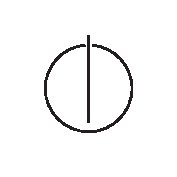
\includegraphics[width=2.4cm]{tum-info-logo}
\end{center}

\newpage

%%%%%%%%%%%%%%%%%%%%%%%%%%%%%%%
% R�ckseite Deckblatt

\thispagestyle{empty}
\cleardoublepage

%%%%%%%%%%%%%%%%%%%%%%%%%%%%%%%
% Erste Seite (Titelblatt)

\thispagestyle{empty}

\begin{center}

    
\includegraphics[width=3cm]{tum-logo}\\
    \vspace{.5cm}
    {\Large \sc Technische Universit�t M�nchen}\\


    \vspace{.5cm}

    {\huge \sc Fakult�t f�r Informatik\\[1mm]}


    \vspace{1cm}

    {\Large \textbf{Diplomarbeit in Informatik}}\\ % oder SEP etc.

% Thema bzw. Titel der Arbeit  (In der Sprache, in der die Arbeit verfasst wurde)
    \vspace{1.5cm}
    {\huge \textbf{Ein Lorem-Rahmenwerk}}\\ % bei langen Titeln ggf. Schriftgr��e herunter setzen
    \vspace*{3mm}
    {\huge \textbf{f�r Ipsum-Systeme}}\\
    \vspace*{3mm}
    {\huge \textbf{-- ein Dolor-Ansatz}}\\

% die englische bzw. deutsche Entsprechung des Titels
    \vspace{1cm}
    {\huge \textbf{A Lorem Framework}}\\ % bei langen Titeln ggf. Schriftgr��e herunter setzen
    \vspace*{3mm}
    {\huge \textbf{for Ipsum Systems}}\\
    \vspace*{3mm}
    {\huge \textbf{-- a Dolor Approach}}\\
    \vspace{1cm}

    \parbox{1cm}{
      \begin{large}
        \begin{tabbing}
          Bearbeiter: \hspace{1.5cm}
            \=Vorname Nachname\\[2mm]
    Aufgabensteller: \>Prof. Dr. Dieter Kranzlm�ller\\[2mm]
    Betreuer: \>MNM-Team-Betreuer 1\\ % alphabetische Reihenfolge (Nachname)
    \>MNM-Team-Betreuer 2\\
    \>Externer Betreuer 1 (Firma)\\[5mm]
    Abgabedatum: \> 7. Juli 2077\\
        \end{tabbing}
      \end{large}
    }\\

    \vspace{.3cm}

    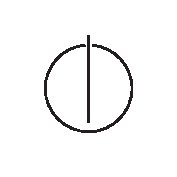
\includegraphics[width=2.4cm]{tum-info-logo}

\end{center}
 % Titelbl�tter TUM - auskommentiert lassen falls LMU-Arbeit
    \thispagestyle{empty}
    \cleardoublepage
    %
% LaTeX-Rahmen f�r Arbeiten am Lehrstuhl Hegering
%
% Harald Roelle, 2001, 2002
%
% basierend auf Arbeiten von Helmut Reiser, Boris Gruschke und Stephen Heilbronner
%

\newpage

\thispagestyle{empty}

\begin{large}

\vspace*{2cm}

\noindent
Hiermit versichere ich, dass ich die vorliegende Masterarbeit
selbst�ndig verfasst und keine anderen als die angegebenen Quellen
und Hilfsmittel verwendet habe.

\vspace{2cm}

\noindent
M�nchen, den 29. September 2017

\vspace{3cm}

\hspace*{7cm}%
\dotfill\\
\hspace*{8.5cm}%
\textit{(Unterschrift des Kandidaten)}

\end{large}
 % Erkl�rung (Arbeit selbstst�ndig verfasst) - auskommentieren falls TUM-Arbeit
%    \begin{large}

\vspace*{2cm}
\noindent
Ich versichere, dass ich diese Diplomarbeit % (bzw. Master's Thesis)
selbst�ndig verfasst und nur die angegebenen Quellen und Hilfsmittel verwendet habe.

\vspace{2cm}

\noindent
M�nchen, den 7. Juli 2077

\vspace{3cm}

\hspace*{7cm}%
\dotfill\\
\hspace*{8.5cm}%
\textit{(Unterschrift des Kandidaten)}

\end{large}
 % Erkl�rung (Arbeit selbstst�ndig verfasst) - auskommentiert lassen falls LMU-Arbeit
    \thispagestyle{empty}
    \cleardoublepage
    \begin{center}
    \textbf{Kurzzusammenfassung}
\end{center}

\noindent Im Rahmen dieser Arbeit wird untersucht, welche Teile von 3D Objekten als visuell interessanter empfunden werden als andere und wie sich die \textit{wahrgenommene Wichtigkeit} auf der Oberfl\"ache solcher Modelle verteilt. Zwei grunds\"atzlich verschiedene L\"osungsans�tze zu dieser Frage werden zu Hilfe gezogen. Es werden automatisch, anhand eines mathematisch begr\"undeten Prozesses errechnete Verteilungen von Wichtigkeit betrachtet. Mit diesen Ergebnissen werden Verteilungen wahrgenommener Wichtigkeit verglichen, welche durch direkte Nutzer-Interaktion mit einer Auswahl-Applikation entstanden sind, die im Rahmen dieser Arbeit erstellt wurde. Das Ziel dieser Arbeit ist das Bereitstellen einer Grundlage von Daten, welche den Anfang einer Evaluation von Unterschieden dieser beiden Vorgehensweisen erm\"oglicht.

32 Nutzer nahmen bei der Studie teil, welche durchgef\"uhrt wurde um die Grundlage f\"ur diese Diskussion zu schaffen. Die Teilnehmer nutzten die im Rahmen dieser Arbeit erstellte Software um Punkt-weise Teile von 3D Objekten, die sie als interessant empfanden, zu markieren. Gleichzeitig wurde ein grundlegendes Differenz-Ma{\ss} entwickelt, welches etwaige Unterschiede beschreiben soll. Dieses hat zum Ziel, eine Prozentzahl als Ergebnis zu liefern, welche beschreibt wie stark die durchschnittliche Nutzer-Auswahl von den vorab errechneten Ergebnissen abweicht.

W�hrend eindeutige \"Ahnlichkeiten erkennbar sind und diese sich auch in den Kennzahlen widerspiegeln, besteht diese Evaluation mehr auf qualitative Beschreibungen von Tendenzen und Mustern, da eine fundierte, umfassende Analyse von Unterschieden solcher Datentypen den Rahmen dieser Arbeit gesprengt h\"atte.

\vspace*{1.5cm}

\begin{center}
    \textbf{Abstract}
\end{center}

\noindent The subject of this work is to inspect which parts of 3D objects are visually interesting, which are not, and how \textit{perceived importance} is distributed on the surface of such models. Two fundamentally different approaches to this question are compared in this work. First, \textit{importance maps} computed by an automated, mathematically founded procedure are considered. Second, distributions of perceived importance, based on direct user input, gathered from an application based on virtual reality technology, are considered. The goal of this work is to collect enough data to start an evaluation of differences between the results of these two approaches.

In order to establish a foundation of this discussion, a user study was conducted with 32 participants. They would each use the software developed in the scope of this work to select parts of objects they deemed \textit{interesting}. Beforehand, a basic measure of difference was conceptualised in order to describe differences that were speculated to be found. The goal was to compute one percentage-ratio which, based on vertex-wise comparison of importance values provided by user input and computation, indicates how much the user selection differs from the results of computation.

While there are clear similarities, this evaluation os more based on observation of tendencies and patterns since a sound, exhaustive analysis of differences in such types of data would have gone beyond the scope of this work.

\newpage
 % Abstract
    \thispagestyle{empty}
    \tableofcontents % Inhaltsverzeichnis

% ---------------------------------------------------------------
\mainmatter % die eigentliche Arbeit

	\chapter{Introduction}
\label{sec:introduction}

Beginning in the 1950's, virtual reality technology \cite{steuer1992defining} has been continuously researched and improved and its professional relevance is becoming ever more present today. There is a plentitude of recent works showing that it bears great potential and positive possible contributions to architecture and construction \cite{sampaio2014application}, \cite{le2015social}, \cite{stouffs2013happening}, healthcare and psychotherapy \cite{baus2014moving}, \cite{merians2014rehabilitation}, \cite{de2014healthcare}, engineering and industrial design \cite{marks2014towards}, \cite{wendrich2016hybrid}, gaming and home entertainment \cite{valente2016live}, \cite{zyda2005visual} and education \cite{merchant2014effectiveness}, \cite{ott2015literature}. One must also consider that this technology can help gaining new insights and open up new perspectives into greater, more abstract matters of social, environmental and economic manner \cite{ovtcharova2015innovation}, \cite{nguyen2016applying}. 

With resources such as memory and computing power becoming more and more available at ever-increasing rates, 3D objects and their mesh representations are constantly growing in complexity and size, in terms of shaders, texture maps as well as the sheer number of vertices. Still, many professional applications revolving around interaction with such models require means of displaying them in real-time without significant perceived loss of quality to ensure a smooth and fast workflow. This is where mesh simplification and segmentation plays an important role \cite{wei2010feature}, \cite{shaffer2001efficient}, \cite{zhao2012saliency} etc.

This issue becomes even more pressing in a professional, commercial context where access to state of the art, high-performance graphic processing units or render farms is not a given for everybody. With less computing power available, means of user-oriented, real-time rendering are of vital importance to a fast and unimpeded way of working on 3D assets.

Little has been done so far concerning research on \textit{mesh saliency} on a vertex level in a virtual reality environment. Whether saliency maps computed via known methods affect user behavior immersed in VR scenes at all, or to which extent has not been investigated in a vertex selection scenario. Furthermore, as of now, the effect on perceived visual quality of saliency-based object simplification as well as user behavior when given the opportunity to declare salient regions themselves is barely touched on at all.

For the selection of parts of objects which seem important to beholders, I was able to use the Virtual Reality and Visualisation Centres five-sided projection installation at the Leibniz Supercomputing Centre in Munich. This installation creates interactive, immersive virtual reality environments via multiple projectors and tracking sensors. Users only need to wear a lightweight pair of stereo shutter glasses that are synchronized with the projectors and thus can seperate two images for the spectator - one for each eye. The glasses are equipped with an electromagnetic tracking system so that their exact position, orientation and tilt can be captured in real-time, allowing the computation of the users perspective in 3D scene at any time. Based on this perspective, the projectors use the walls as projection surfaces and throw live images resembling what the user would see if he/she were physically in the virtual scene onto the walls. The projection installation grants a virtual reality experience which is enhanced by the fact that the user only needs to wear a pair of glasses instead of a fully sized headset. From a user perspective, another advantage of such a setup is the fact that there are no cables connected to the glasses which can evoke a feeling of inhibition or the constant worry of stumbling over or accidentally damaging the cables.

% Überleitung hier: Was passiert generell?
% im Absatz oben checken ob eletromagnetic trackers stimmt

Finally, it is worth noting that the effect on perceived quality of objects in 3D scenes that can possibly achieved through saliency-based simplification is not limited to virtual reality applications. Long-term goals of efficiency and optimization will continue to be accompanied by the need for semi-automatic complexity reduction of objects without a great loss of visual appeal, regardless of the type of media they will be presented on. So the best case outcome of this work is to find possible approaches to identifying segments of objects which are of high importance to the average beholder based on the immersive nature of the selection process of said segments.

% Kapitel der Arbeit beschreiben

	\chapter{Related work}
\label{sec:related_work}

This section is subdivided into two parts. First, publications discussing \textit{mesh saliency}, a technique used term to predict regional percieved importance of digital representations of real-world (or synthetic) objects as well as 2D images, will be presented and briefly described. The second section will provide a look into human behavior, based on cognition and outside stimuli in virtual reality environments. These two sets of scientific works will provide a solid knowledge of terms and methods commonly used in this field and describe the current state of the art.

\section{Mesh saliency and human perception}
\label{sec:mesh_saliency_and_human_perception}

Research on what human perception guides us to focus our attention on when presented with an 3D representation of an object was begun just past the year 2000 and has been a continuous effort ever since. One commonly cited publication in this field is Lee \textit{et al.} \cite{lee2005mesh}. Based on low-level human visual attention \cite{koch1987shifts}, it introduces the term \textit{mesh saliency}, a measure for regional based importance of 3D meshes, and also presents a way to compute it. This fully automatic process successfully predicts  what would be classified by most observers as prominent, visually interesting regions on a mesh, thus allowing mesh operations such as simplification \cite{cignoni1998comparison} and segmentation \cite{shamir2008survey} to produce results that are more appealing to the beholder.

\begin{figure}[htb]
  \centering
  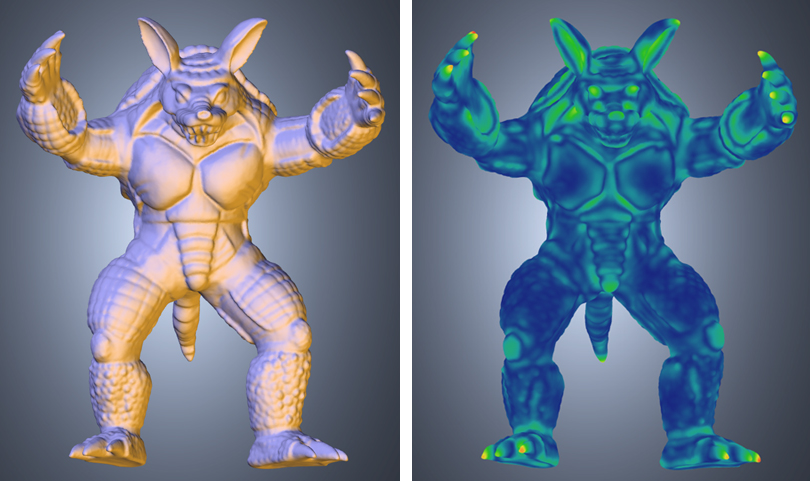
\includegraphics[width=1.0\textwidth]{arma.png}\\ % PNG-File
  \caption{A model and its computes mesh saliency map. Published by Lee \textit{et al.} \cite{lee2005mesh}. Bright colors (yellow and red) indicate high saliency values for their respective vertices, dark colors (shades of blue) indicate low values.}\label{fig:lee_arma_map}
\end{figure}

The model for computing \textit{mesh saliency} is based on a center-surround comparison of local curvature. It is scale-dependent on a \textit{saliency factor} $\varepsilon$, which is based on the diagonal of the objects bounding box, and is able to identify salient features of a mesh, depending on their surrounding area. Geometrically complex regions, for example a large patch containing lots of bumps of similar size, will be rightfully dismissed as, in most cases, regions that are not interesting from a human perceptional stance.

Taking a closer look at the basic formula through which saliency for any vertex of a mesh can be computed according to Lee \textit{et al.} helps understanding the underlying concept. As a first step, the mean curvature map for a mesh, describing mean local curvature values on a point-level for each of its vertices, needs to be calculated via commonly known approaches such as \cite{taubin1995estimating}. The resulting mean curvature map $\mathscr{C}$ defines a mapping from each vertex of a mesh to its mean curvature $\mathscr{C}$(\textit{v}). Using a distance measure such as the Euclidean or geodesic method, one can compute the neighbourhood \textit{N}(\textit{v},$\sigma$) of a vertex \textit{v} which then defines a set of points within a distance $\sigma$. The Euclidean appraoch was used in Lee \textit{et al.} and subsequently in the formula below.
Using these definitions, the authors denote the Gaussian-weighted average of the mean curvature by G($\mathscr{C}$(\textit{v}),$\sigma$) and present the following way of computing it.

\begin{align*}
G(\mathscr{C}(v),\sigma) &= \frac
	{
		\sum_{x \in N(v,2\sigma)}
			\mathscr{C}(x)exp	-||x-v||^2 \backslash(2\sigma^2)
	}{
		\sum_{x \in N(v,2\sigma)}
			exp -||x-v||^2 \backslash(2\sigma^2)
	}
\end{align*}

For computation of the Gaussian-weighted average, a cut-off factor for the filter is assumed at a distance of 2$\sigma$, in other words twice the distance that a vertex can have to another vertex to still be considered in its neighbourhood.
Based on these definitions, the saliency $\mathscr{S}$(\textit{v}) of a vertex \textit{v} is defined as the abslute difference between the Gaussian-weighted averages, as seen in the formula below.

\begin{align*}
\mathscr{S}(\textit{v}) &= |\textit{G}(\mathscr{C}(\textit{v}),\sigma) - G(\mathscr{C}(\textit{v}),2\sigma)|
\end{align*}

In order to get more refined results, one can conduct multiple computations of \textit{mesh saliency} with different values for $\sigma$. Lee \textit{et al.} use the previously mentioned \textit{saliency factor} $\varepsilon$ with $\varepsilon \in [2,6]$ in their paper, to generate multiple values for $\sigma$.

The concept of \textit{mesh saliency} has since been refined, augmented and adapted to serve as a basis for a multitude of specific use-cases and applications. When processing single vertex saliency, Wu \textit{et al.} \cite{wu2013mesh} took into consideration not only the curvature of the region surrounding the vertex, but also the global context of it. In other words, for each vertex to be attributed a value describing its saliency, its \textit{global rarity}, derived from comparing its features to those of every other vertex of the object, is computed. They performed a user study in which they had participants choose one out of two saliency maps for a set of objects, presented in a random order. One map was generated using their approach, the other one with the model presented in Lee \textit{et al.} Participants were asked to pick the one that was a closer representation of what they would have considered interesting regions and features. Since their method got picked in almost 58 per cent of cases, while the results produced by the model presented in Lee \textit{et al.} were favored in about 42 per cent, this can be considered a true improvement of the way \textit{mesh saliency} can be computed.

One approach to improve the method of finding salient elements in 2D images relied on paying extra attention to depth-information in \cite{ciptadi2013depth}. In this work, Ciptadi \textit{et al.} found that better results in terms of automatic identification of objects and surfaces could indeed be achieved this way. Transferring these insights into a 3D context is easy since visually complex models often base on multiple image-maps describing, among other information, depth values on the surfaces of the model.
In \cite{potapova2011learning}, the authors took a more task-driven approach to contribute to the concept of \textit{saliency}. Gathering colour- and depth information about real-world scenes using a Kinect sensor, they extracted semantic cues about surface heights, relative surface orientations and occluded edges. Based on that data, they computed combined saliency maps which allowed them to assign real-world objects to four different categories, enhancing ways a robotic system can interact with them, providing the best possible points where the objects can be grasped and whether they are in reach at all or not (due to occlusion by other objects).

Another recent work aimed at identifying single, distinct elements and objects of 3D models was presented in \cite{koschan2003perception} by Koschan \textit{et al.} The authors propose a segmentation algorithm that utilises a human perception phenomenon known as the \textit{minima rule} which suggests that contours of negative curvature minima can serve as boundaries of disjunct visual parts or elements. Another detailed comparison between automatically detected points of interests and what participants in a study actually declared as visually interesting points was drawn by Dutagaci \textit{et al.} in \cite{dutagaci2012evaluation}.

To verify the practical relevance of identifying salient regions and features on 3D meshes, Howlett \textit{et al.} \cite{howlett2005predicting} conducted a user study on whether it is possible to determine such features in advance. Based on observations gathered from eye-tracking device based user studies, they concluded that, especially with natural objects (animals, humans etc.), this was indeed the case. On top of that, they also reported a significant increase in visual fidelity on objects which were simplified based on saliency weight-maps, according to reports of study participants. Furthermore, in \cite{kho2003user} the authors used user-guided simplification to preserve higher levels of detail in areas of 3D objects that people deemed important to the recognisability of the object. After performing mesh simplification according to \cite{garland1997qslim}, enhanced by taking user-derived weight maps into account, the authors observed what they described as perceptually improved approximations of input objects.

In another highly noteworthy work by Munaretti \cite{munaretti2007perceptual}, the concept of \textit{mesh saliency} was extended to deformable, i.e. animated objects. The author presented a way to generate so-called \textit{multi-pose saliency}, a combination of multiple saliency maps compoted for static poses of a mesh. These static meshes can also be interpreted as keyframed poses for dynamic deformation, which makes this work a potentially outstanding contribution to any field where 3D objects are being animated.

The author found a remarkable improvement of the original way of computing \textit{mesh saliency} as presented by Lee \textit{et al.} by using geodesic distance \cite{surazhsky2005fast} instead of euclidean distance when comparing local curvature values and implemented a way to compute multiple saliency maps for different levels of detail.

\section{Human attention in Virtual Reality}
\label{sec:human_attention_in_virtual_reality}

While navigation in virtual reality space via a traditional desktop setup with input devices such as a mouse and a keyboard still seems to allow users to perform better in basic tasks such as navigation, they generally perceived interaction via a head-mounted display more natural and intuitive \cite{santos2009head}. It is worth noting though, that this work evaluated a series of user studies described in their respective papers which were published between 1997 and 2006. Thus, it is safe to assume that recent VR technology would get much better results in comparison. This was hinted at in the paper multiple times, mentioning the idiosyncrasies of the equipment used in the studies.
The main tasks in the studies described in this paper included navigation (both in small and large-scale virtual environments), searching for certain objects, physically replicating simple virtual sculptures as well as generic volume visualisation tasks (identification, judgement of size, shape and connectivity). Regarding navigation, the authors concluded that during the six considered studies, slightly faster or equal completion times between VR and desktop setup users could be observed. Results for search tasks were found to be more varied. One study reportedly concluded that desktop users were faster, another one stated the opposite. Visualisation tasks such as size estimations were fulfilled with better results by users in a fully immersive virtual environment compared to participants using a head mounted VR display \cite{qi2006comparison}. This is an interesting find for this work since this user study was conducted with the help of so-called fish tank VR \cite{ware1993fish}. This setup, due to the lightweight stereoscopic glasses and almost unrestricted freedom of movement, resembles a very basic variation of the kind of immersive experience that can be achieved with the use of a multi-wall projection installation which I had access to for this work.

Another, in the context of this work, very relevant study described in the paper above is \cite{mizell2002comparing}. This work, aiming at finding measurable advantages of immersive virtual reality (IVR) over conventional display methods within the context of complex 3D geometry, had users cloesly observe sculptures consisting of more or less randomly bent rods of equal thickness. The users - grouped into IVR and desktop users - were asked to physically replicate the fairly complex object with real, easily deformable leaden rods while looking at the virtual object. The paper describes two studies, in one of wich the IVR setup was a multi-sided projection installation, allowing the users to view the geometric data from effectively every possible position and angle while the desktop user group had to use a joystick or control pad for navigation. It reports that IVR users performed consistently superior regarding both time and error-rate. This suggests that immersive virtual technology might be able to offer a more precise understanding of complex geometric data which is a compelling assumption regarding this work.

With the ambition to develop a predictive model for the positive outcome using a VR setup can have compared to its expenses, Pausch \textit{et al.} \cite{pausch1997quantifying} found that, while not being being able to help users perform search tasks in virtual space faster than with a desktop setup, users with a head-mounted display were able to complete the tasks with more certainty. They spent significantly less time re-examining areas, which they commonly did with the desktop setup - up to 41\% more time. The task users were given in this work was to find a specific letter hidden on the walls of a virtual room which were textured with evenly spread sets of letters, or confidently declare that the letter wasn't present. The target letter was not actually present in the room in 50\% of the tests. Based on the observation that VR users in this study barely spent any time rescanning parts of the virtual room, the authors assumed that a VR setup can have a greatly beneficial impact on systematic search tasks. They based this on the fact that spatial understanding and navigation skills are naturally very well developed parts of human cognition and proposed that the immersive experience did such a sufficiently well job at mimicking a real life environment that these skills could be used to a greater extent than in a desktop setup. Again, this is further reason to be optimistic about finding interesting patterns in what users in a VR setup find to be highly significant regions of 3D objects.

Taking a step back towards the basics of human attention in 3D space, in 1998, Atchley \textit{et al.} \cite{atchleyattentional} conducted four experiments addressing attention in 3D scenes on a very basic level. Participants were shown simple scenes, each containing sets of six short lines. The scenes were arranged on four different depth planes, one behind the other, and displayed on a stereographic display. The basic task given to participants in all of the experiments was to focus a briefly visible colour singleton on a specific, previously cued depth plane. One of the lines on the indicated plane would change its colour for 100 milliseconds and participants had to correctly say whether it was tilted to the left or the right. To determine the time it takes to shift attention from one plane to another, for some user groups, the colour singleton would appear in a plane other than the previously hinted one. To further track speed and accuracy of attention focus, a distraction element (one additional line changing its colour simultaneously to the target line) was shown to some participants, sometimes in the \textit{target plane}, sometimes in a different one. From their observations, the authors gathered that depth-plane attention can be successfully guided and that distraction elements appearing on the \textit{target plane} significantly interfered with the users' ability to give correct answers, while such elements appearing on other planes had virtually no impact on results.

Taking the effort of tracking attention a step further into virtual reality context, Lee \textit{et al.} \cite{lee2007real} accomplished just that on an object basis. They presented a framework capable of such a task, both bottom-up (stimulus-driven) and top-down (goal-directed). Based on pixel-level saliency maps, computed via known methods, similar maps for multiple objects in the scene are generated, allowing predictions on which objects will more likely to be focused first by users. Using the method presented in this paper, object-level saliency maps can be computed in real-time, depending on the users dynamic position and orientation within the scene. The authors exploited knowledge of human cognition which suggests that attention is object-based \cite{o1999fmri} and, using a monocular eye tracking device, compared the results of estimated object-level saliency maps to the behavior of participants in their study. They dynamically assigned saliency values to each object and, depending on how many of the objects with the highest values (first 1, 2 or 3) were taken into consideration, observed estimation accuracies ranging from about 50 per cent to up to nearly 95 per cent. As one can imagine, accuracy values were the highest when users were given a task, for example finding a certain object within the scene. This shows that attention in virtual space can be tracked and accurately predicted on object level.

In 2012, Y. Kim \textit{et al.} \cite{chen2012schelling} conducted a study that relied on an eye-tracking system to compare previously computed saliency maps to eye movements of participants, aiming at comparing the computer generated saliency map with user input describing regional importance of 3D objects. The authors based the computation of mesh saliency maps on the work by Lee \textit{et al.} \cite{lee2005mesh}. They then introduced a normalized, chance-adjusted saliency in order to evaluate the correlation between point-wise mesh saliency values and the users' eye fixations on 2D rendered images of 3D objects, each visible for five seconds. They concluded that the computational model of mesh saliency has better correlation with human eye fixation points than both a randomly model as well as another curvature-based model during this specific timespan. This suggests a basic correlation between mesh saliency maps and input gathered from tracking human vision. However, since 2D images were used during this study and there was no form of interaction whatsoever, lots of ways to validate the relevance of mesh saliency are still untouched.

%    \chapter{Finibus Bonorum et Malorum}

Lorem ipsum dolor sit amet, consectetuer adipiscing elit. Nullam et lectus ac lacus bibendum ullamcorper. Sed ante neque, scelerisque eu, sodales quis, elementum nec, risus. Aliquam erat volutpat. Suspendisse potenti. Praesent erat justo, viverra sed, dignissim ut, tempus eget, orci. Morbi luctus ultrices tortor. Maecenas sit amet enim. Morbi facilisis fringilla nunc. Fusce venenatis nunc a nunc. Quisque interdum pretium erat. In mattis feugiat sapien. Aliquam erat volutpat. Proin pellentesque ullamcorper risus. Integer at risus ut velit eleifend sagittis.

\section{In adipiscing purus et purus}

Vestibulum eu velit \cite{han99}. Donec pharetra feugiat elit. Morbi vitae arcu. Sed dignissim, lectus at ultricies fringilla, mauris mi eleifend mi, nec varius ipsum nunc a enim. Vivamus quis libero a erat varius accumsan. Nullam porttitor, est vitae dignissim eleifend, lacus mi semper justo, elementum imperdiet ante nibh sed nisl. Pellentesque suscipit venenatis ipsum. Suspendisse ultricies elit et neque. Sed risus erat, vehicula eget, vulputate sit amet, viverra sit amet, arcu. Integer malesuada risus vitae est. Donec vulputate, enim a laoreet vehicula, est magna vulputate justo, ut congue sapien mi gravida arcu. Curabitur luctus sapien id orci. Maecenas pulvinar, dolor id placerat convallis, mi metus fringilla enim, eu dignissim urna justo sollicitudin nibh. Vestibulum tellus nisi, nonummy vitae, aliquet a, vehicula et, justo.

\subsection{das sollte 1.1.1 sein}
asdf1234

\subsection{Ulauts}
w\"ork \"Auglein

Donec viverra tortor non lectus. Vestibulum vel nulla ac sapien tristique imperdiet. Sed neque. Suspendisse porta risus nec mi. Nulla id orci. Donec nunc dolor, ullamcorper sit amet, imperdiet vitae, blandit et, lacus. Cum sociis natoque penatibus et magnis dis parturient montes, nascetur ridiculus mus. Suspendisse potenti. Ut nibh. Cras enim. Mauris a ligula scelerisque ligula dictum cursus. Proin malesuada massa non nulla. Praesent imperdiet massa eu justo.

%Grafik aus PNG-File - bei dieser Variante darauf achten, dass die Grafik in ausreichender Aufl�sung vorliegt (so dass auch nach Skalierung >300dpi im Ausdruck erreicht werden) 
\begin{figure}[htb]
  \centering
  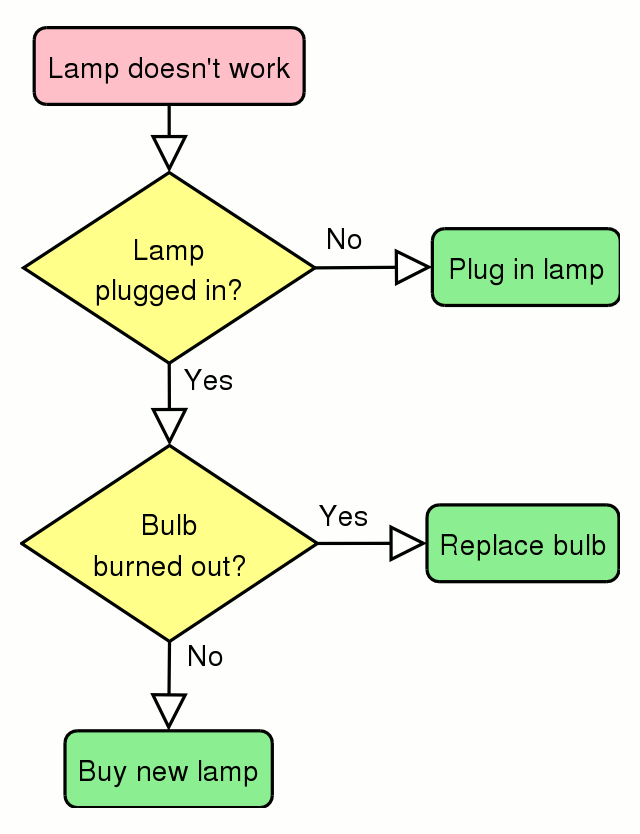
\includegraphics[width=.4\textwidth]{LampFlowchart}\\ % PNG-File
  \caption{Nulla interdum aliquam leo}\label{fig:LampFlowchart}
\end{figure}


Vestibulum ante ipsum primis in faucibus orci luctus et ultrices posuere cubilia Curae (vgl. Abbildung \ref{fig:LampFlowchart}); Curabitur mauris urna, tincidunt eget, porttitor in, lacinia vel, massa. Integer nonummy, elit at ullamcorper facilisis, massa sem elementum sapien, non malesuada ipsum lacus sed enim. Cras nec eros ut sapien sodales scelerisque. Sed quam. Suspendisse potenti. Nunc eu tortor. Nam nisi arcu, mattis ut, vehicula et, tristique in, erat. Class aptent taciti sociosqu ad litora torquent per conubia nostra, per inceptos hymenaeos. Nullam justo. Integer eget erat at mauris tristique ultrices. Sed ullamcorper vulputate velit. Vivamus blandit erat non erat luctus venenatis. Mauris elementum semper nunc. Cras pellentesque tristique nulla. Pellentesque metus. Mauris semper mi quis pede. Proin vel tellus.

Maecenas euismod, orci in mollis scelerisque, turpis elit lobortis nunc, a venenatis nisl orci quis nibh. Duis tincidunt dictum elit. Nulla sodales est nec nisi. Phasellus consectetuer suscipit urna. Nulla augue. Pellentesque tincidunt pellentesque diam. Etiam iaculis. Cras aliquet metus sed est. Cras egestas, nibh nec commodo suscipit, mauris dolor blandit dolor, id egestas lorem nibh eu nisl. Sed tempor tempor lorem. Donec fringilla luctus quam. Nam metus magna, varius non, tempor eget, rutrum quis, velit. Maecenas sit amet neque id tellus venenatis scelerisque. Donec sed purus. Quisque eu quam a augue consequat consequat.

\section{Etiam blandit molestie ligula}

Proin pharetra ultrices enim. Maecenas dui. Mauris est eros, posuere vitae, sagittis quis, tempus ut, mauris. Fusce congue, augue imperdiet tincidunt volutpat, justo metus tristique lacus, eu ultrices mauris mi ac tellus. Praesent porttitor accumsan erat. Quisque lacinia mollis turpis. Suspendisse potenti. Morbi eu urna vel purus congue accumsan. Aliquam consectetuer nulla nec augue. Nam fringilla nisi nec felis. Donec nibh tellus, consequat quis, cursus sed, vulputate eu, orci. Donec vulputate, elit vel iaculis hendrerit, augue augue congue erat, vel vestibulum tortor dui a diam (vgl. Abbildung \ref{fig:BurgerFlowchart}). Etiam vel lorem a libero feugiat feugiat. In blandit est a est. Nulla interdum pharetra nulla. Nullam eu ipsum.

%Grafik aus PDF-File - diese Variante ist vorzuziehen, da sie die Einbundung echter Vektorgrafiken erm�glicht 
\begin{figure}[htb]
  \centering
  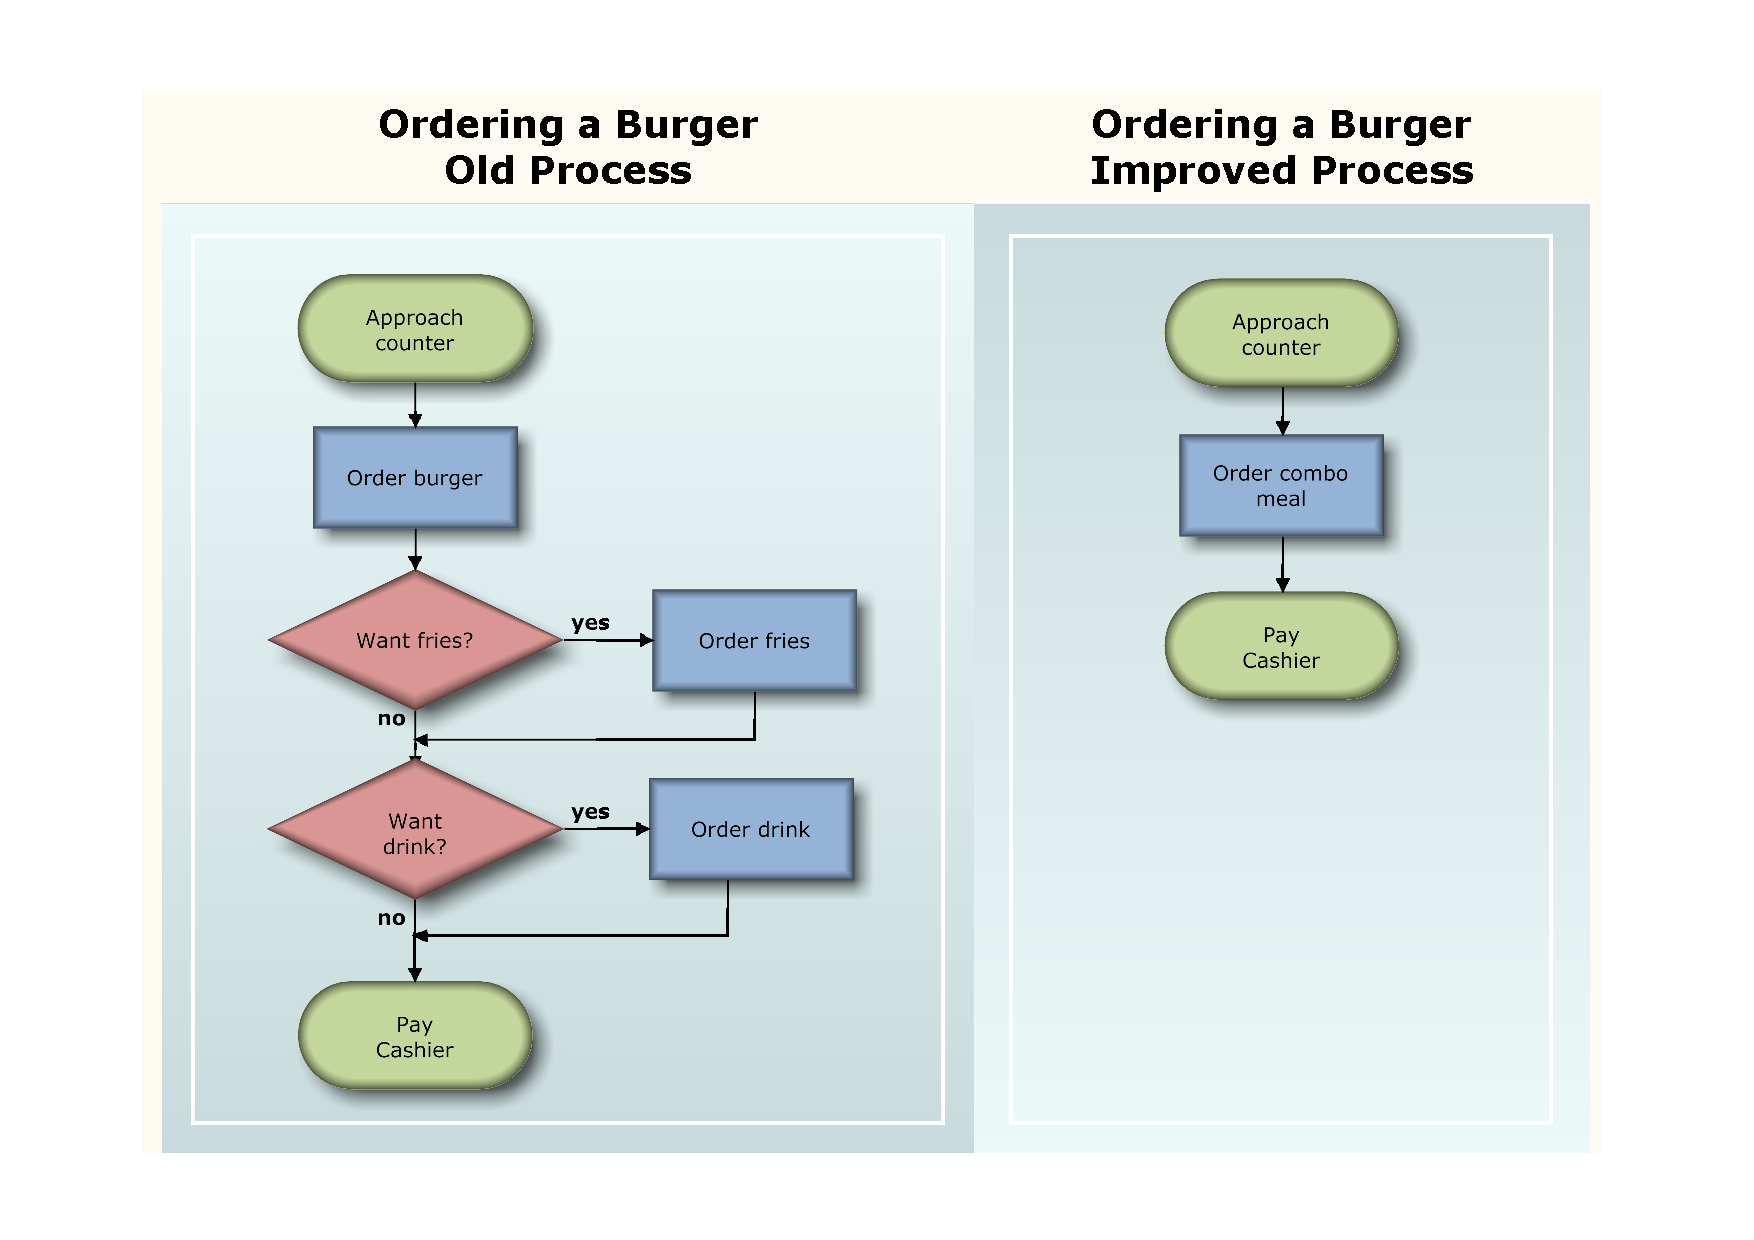
\includegraphics[scale=.6]{BurgerFlowchart}\\ % PDF-File
  \caption{Donec tempor leo a massa \cite{scrguide07}}\label{fig:BurgerFlowchart}
\end{figure}

Quisque ligula orci, accumsan vel, molestie ac, lacinia non, lorem . Fusce nonummy. Cras mattis, elit ac tempor congue, ante arcu porta justo, at rhoncus sapien erat vel dui \cite{kop02}. Phasellus vestibulum, turpis non tempor vehicula, quam lacus accumsan dolor, id dictum magna magna eu neque. Sed suscipit placerat odio. Sed et sem. Mauris vel tortor a nisl egestas vulputate. Aliquam facilisis luctus nibh. Maecenas vel lectus sed urna viverra pretium. Aenean malesuada nibh sed ipsum. Fusce vel augue. Mauris eget massa. Class aptent taciti sociosqu ad litora torquent per conubia nostra, per inceptos hymenaeos. Etiam nec justo eu purus ultricies mattis. In leo ante, adipiscing sit amet, ultrices at, ultrices et, nulla. Mauris quis odio. Donec sollicitudin rutrum sapien. Aliquam eget ante a dui euismod porttitor. Donec commodo scelerisque purus. Sed magna.

Cras gravida. Praesent posuere lacus ut tellus. Nunc tempor dapibus urna. Proin sit amet velit ut urna lobortis ultrices. Suspendisse potenti. Maecenas est libero, condimentum in, mattis a, viverra in, sem. Sed nec pede. Fusce risus magna, porta eu, rhoncus vel, facilisis at, risus. Donec commodo viverra neque. Donec ultrices neque vitae justo. Nulla et magna. In condimentum tellus vitae erat. Quisque nec odio.


Nullam consectetuer risus vitae orci. Aliquam fermentum leo sit amet nulla laoreet hendrerit. Maecenas tempus, neque eu posuere vestibulum, pede eros adipiscing augue, pulvinar ullamcorper lectus lectus et tellus. Donec at velit at velit pellentesque sagittis. Vestibulum ultricies ultrices mi. Vestibulum accumsan dictum ligula. Ut lobortis, odio ut semper vehicula, nibh quam semper nisi, sed adipiscing purus lectus et sem. Mauris nisl est, scelerisque ut, ultrices nec, faucibus vitae, nulla. Nulla nisi. Suspendisse potenti. Etiam ultrices commodo odio. Quisque turpis purus, mollis sed, pretium quis, volutpat et, neque. Nam a sapien eget neque consectetuer ornare. Pellentesque felis metus, pellentesque quis, volutpat rhoncus, laoreet id, nunc. Duis egestas, felis et luctus vestibulum, velit nunc luctus felis, non tempor justo ligula et nulla. Vestibulum, Abbildung \ref{fig:tabelle}, est. Nulla aliquam eleifend justo.

%Tabellen im Regelfall auch in eine Figure-Umgebung setzen - Verwendung von Table-Umgebung lohnt nur bei sehr vielen Tabellen
\begin{figure}[htb]
  \centering
  \begin{tabular}{|l|c|}
    \hline
    \textbf{tempus} & \textbf{risus} \\ \hline
    ultrices & pellentesque \\
    rhoncus & egestas \\
    \hline
  \end{tabular}
  \caption{Aliquam fermentum}\label{fig:tabelle}
\end{figure}

Class aptent taciti sociosqu ad litora torquent per conubia nostra, per inceptos hymenaeos. Lorem ipsum dolor sit amet, consectetuer adipiscing elit. Sed auctor urna quis turpis. Suspendisse potenti. Donec tempus gravida ante. Nulla magna velit, condimentum et, pharetra sollicitudin, tincidunt et, nibh. Donec tincidunt, leo a facilisis consectetuer, quam diam cursus nibh, vitae porttitor lacus dolor in lacus. Nulla id nulla in dolor adipiscing posuere. Proin sagittis mattis dui. Maecenas neque arcu, ornare a, gravida et, posuere ut, massa. Donec congue odio ac enim. Nam malesuada sapien sit amet ante. Donec ullamcorper pulvinar dolor. Fusce posuere tellus.

\section{Ut venenatis mi id orci}

Class aptent taciti sociosqu ad litora torquent per conubia nostra, per inceptos hymenaeos. Ut quam odio, luctus gravida, aliquam eu, fringilla a, nulla. Nulla facilisi. Aliquam tincidunt porta urna. Nulla facilisi. Cras pellentesque cursus risus. Quisque semper imperdiet ante. Donec erat magna, sagittis vitae, convallis ut, tincidunt et, lectus. Mauris vulputate tincidunt mi. Integer diam enim, mollis non, dignissim non, faucibus eu, enim. Aliquam erat volutpat. Sed facilisis sagittis massa. Vivamus vel neque. Donec eu mi. Aenean lobortis. Nullam pulvinar. Mauris vel lorem vel dolor semper volutpat. Nam posuere blandit arcu.

\endinput 


% ---------------------------------------------------------------
\backmatter % ab hier keine Nummerierung mehr
    \listoffigures
    \bibliographystyle{alpha}
    \bibliography{./Bib/metz17}

\end{document}
